\chapter{The Wave Equation}

% ============================================================
\section{The Continuum Wave Equation}
% ============================================================

In the previous chapter we followed a chain of coupled oscillators as the number of masses grew without bound and the spacing between them shrank to zero. In that continuum limit the discrete set of coupled ordinary differential equations collapses into a single partial differential equation. For a stretched string of linear mass density $\rho_L$ under tension $T$, the transverse displacement $\psi(x,t)$ obeys the one-dimensional \emph{wave equation}:
\begin{formula}
\begin{equation}
    \pdv[2]{\psi}{t} = \frac{T}{\rho_L}\,\pdv[2]{\psi}{x}
    \;=\; v_p^{\,2}\,\pdv[2]{\psi}{x},
    \qquad v_p \defeq \sqrt{\frac{T}{\rho_L}}.
\end{equation}
\end{formula}
The constant $v_p$ carries units of velocity and, as the traveling-wave solutions below will make explicit, it is the speed at which disturbances propagate along the string. What makes this equation so central is that it is not special to strings: the very same form governs longitudinal pressure waves in a gas (with $v_p = \sqrt{\gamma p_0/\rho}$), electromagnetic waves in vacuum (with $v_p = c = 1/\sqrt{\mu_0\varepsilon_0}$), and countless other fields. The field $\psi$ is therefore best read as a \emph{generalized displacement} --- a mechanical position, a pressure fluctuation, or a component of $\vect{E}$ --- and everything we prove here transfers wholesale to those settings.

\begin{definition}[Dispersion relation]
Substituting a plane-wave ansatz $\psi \sim e^{i(kx-\omega t)}$ into the wave equation gives a relation between frequency and wavenumber,
\begin{equation}
    \omega^2 = v_p^{\,2}\,k^2 \quad\Longleftrightarrow\quad \omega = v_p\,|k|.
\end{equation}
The linearity of $\omega$ in $|k|$ characterizes a \emph{nondispersive} medium: every wavelength travels at the same phase velocity $v_p$, so an arbitrary pulse propagates without changing shape. Dispersive media, for which $\omega \neq v_p k$, are the exception rather than the rule for the systems considered here.
\end{definition}

Because the wave equation is linear and homogeneous, the superposition principle applies just as it did for the single oscillator: any sum of solutions is again a solution. This licenses two complementary strategies for building the general solution. The first, developed in the next sections, superposes \emph{standing waves} --- spatial mode shapes that oscillate in place. The second, taken up later, superposes \emph{traveling waves} that glide rigidly along the string. A single normal mode of the standing-wave family has the separable form
\begin{equation}
    \psi_m(x,t) = A_m\,\sin(k_m x + \alpha_m)\,\sin(\omega_m t + \beta_m),
    \label{eq:normalmode}
\end{equation}
with $\omega_m = v_p\,k_m$. Each mode carries four parameters: two of them, $k_m$ and $\alpha_m$, are fixed by the two boundary conditions in $x$, while the remaining two, $A_m$ and $\beta_m$, are fixed by the two initial conditions at $t=0$. The full solution is a superposition over all admissible mode indices $m$.

% ============================================================
\section{Standing Waves and Boundary Conditions}
% ============================================================

The boundary conditions are what quantize the string: they select a discrete set of allowed wavenumbers $k_m$ from the continuum, exactly as the walls of a box quantize the modes inside it. We treat the two most important cases in turn.

\subsection{Two Fixed Ends}

The prototypical string has both endpoints clamped, as on a guitar or a piano:
\begin{equation}
    y(0,t) = 0, \qquad y(L,t) = 0 \quad \text{for all } t.
\end{equation}
The condition at $x=0$ forces $\sin(\alpha_m) = 0$, so we may take $\alpha_m = 0$ (any sign is absorbed into $A_m$). With $\alpha_m=0$ the condition at $x=L$ then requires $\sin(k_m L) = 0$, which selects
\begin{formula}
\begin{equation}
    k_m = \frac{m\pi}{L}, \qquad \omega_m = \sqrt{\frac{T}{\rho_L}}\,\frac{m\pi}{L}, \qquad m = 1, 2, 3, \ldots
\end{equation}
\end{formula}
The corresponding mode shape is
\begin{equation}
    y_m(x,t) = A_m\,\sin\!\left(\frac{m\pi x}{L}\right)\sin(\omega_m t + \beta_m).
\end{equation}
The lowest mode $m=1$ fits exactly half a wavelength into the length $L$, so $\lambda_1 = 2L$; the $m$-th harmonic fits $m$ half-wavelengths and has $m-1$ interior \emph{nodes} where the string stays permanently at rest (Figure~\ref{fig:fixed-fixed}). Between the nodes sit \emph{antinodes}, points of maximal oscillation. Because $\omega_m = m\,\omega_1$ is an exact integer multiple of the fundamental, the clamped string sounds a harmonic series --- the reason plucked strings produce a definite musical pitch.

\begin{figure}[ht]
\centering
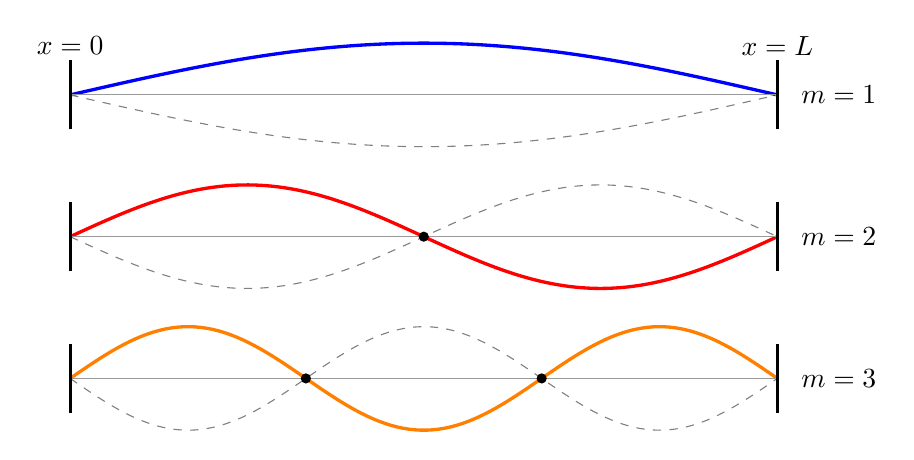
\begin{tikzpicture}
\begin{axis}[
    hide axis,
    width=12cm, height=8cm,
    xmin=-0.08, xmax=1.08, ymin=-3.35, ymax=0.75,
    samples=120, domain=0:1,
    clip=false,
]
    % m = 1
    \addplot[very thick, blue] {0.42*sin(deg(pi*x))};
    \addplot[gray, dashed] {-0.42*sin(deg(pi*x))};
    % m = 2
    \addplot[very thick, red] {-1.15 + 0.42*sin(deg(2*pi*x))};
    \addplot[gray, dashed] {-1.15 - 0.42*sin(deg(2*pi*x))};
    % m = 3
    \addplot[very thick, orange] {-2.30 + 0.42*sin(deg(3*pi*x))};
    \addplot[gray, dashed] {-2.30 - 0.42*sin(deg(3*pi*x))};
    % baselines and walls
    \draw[thin, black!40] (axis cs:0,0) -- (axis cs:1,0);
    \draw[very thick] (axis cs:0,-0.28) -- (axis cs:0,0.28);
    \draw[very thick] (axis cs:1,-0.28) -- (axis cs:1,0.28);
    \draw[thin, black!40] (axis cs:0,-1.15) -- (axis cs:1,-1.15);
    \draw[very thick] (axis cs:0,-1.43) -- (axis cs:0,-0.87);
    \draw[very thick] (axis cs:1,-1.43) -- (axis cs:1,-0.87);
    \draw[thin, black!40] (axis cs:0,-2.30) -- (axis cs:1,-2.30);
    \draw[very thick] (axis cs:0,-2.58) -- (axis cs:0,-2.02);
    \draw[very thick] (axis cs:1,-2.58) -- (axis cs:1,-2.02);
    % node markers
    \node[fill=black,circle,inner sep=1.3pt] at (axis cs:0.5,-1.15) {};
    \node[fill=black,circle,inner sep=1.3pt] at (axis cs:0.3333,-2.30) {};
    \node[fill=black,circle,inner sep=1.3pt] at (axis cs:0.6667,-2.30) {};
    % labels
    \node[anchor=west] at (axis cs:1.02,0) {$m=1$};
    \node[anchor=west] at (axis cs:1.02,-1.15) {$m=2$};
    \node[anchor=west] at (axis cs:1.02,-2.30) {$m=3$};
    \node[anchor=north] at (axis cs:0,0.55) {$x=0$};
    \node[anchor=north] at (axis cs:1,0.55) {$x=L$};
\end{axis}
\end{tikzpicture}
\caption{The first three harmonics of a string clamped at both ends. Solid curves show the extreme displacement; dashed curves the opposite phase. The $m$-th mode has $m-1$ interior nodes (dots) and wavelength $\lambda_m = 2L/m$.}
\label{fig:fixed-fixed}
\end{figure}

\subsection{Mixed Boundary Conditions: One Free End}

Now replace the clamp at $x=L$ with a massless ring free to slide vertically on a frictionless rod. Because the ring has no mass, Newton's second law applied to it reads
\begin{equation}
    m_{\text{ring}}\,\ddot{y}_{\text{ring}} = T\sin\theta = 0 \quad\Longrightarrow\quad \sin\theta = 0,
\end{equation}
where $\theta$ is the angle the string makes with the horizontal at the ring. For small angles $\sin\theta \approx \pdv{\psi}{x}$, so the free end is a \emph{Neumann} boundary on which the slope vanishes:
\begin{fact}
A frictionless massless ring at $x=L$ imposes
\begin{equation}
    \left.\pdv{\psi}{x}\right|_{x=L} = 0,
\end{equation}
so the string meets the rod horizontally. Physically the ring can exert no vertical force, and a nonzero slope would demand one.
\end{fact}
Keeping the fixed end at $x=0$ (which again gives $\alpha_m = 0$), the free-end condition becomes $A_m k_m \cos(k_m L)\sin(\omega_m t + \beta_m) = 0$, forcing $\cos(k_m L) = 0$ and hence
\begin{formula}
\begin{equation}
    k_m = \frac{\left(m - \tfrac{1}{2}\right)\pi}{L}, \qquad m = 1, 2, 3, \ldots
\end{equation}
\end{formula}
The mode shape is
\begin{equation}
    \psi_m(x,t) = A_m\,\sin\!\left(\frac{(m-\tfrac{1}{2})\pi x}{L}\right)\sin(\omega_m t + \beta_m).
\end{equation}
Now only odd multiples of a quarter-wavelength fit into $[0,L]$: the fundamental has a node at the fixed end and an antinode at the free end, giving $\lambda_1 = 4L$ (Figure~\ref{fig:fixed-free}). The allowed frequencies are the odd harmonics $\omega_1, 3\omega_1, 5\omega_1, \ldots$ of a fundamental one octave below that of the doubly clamped string of the same length.

\begin{figure}[ht]
\centering
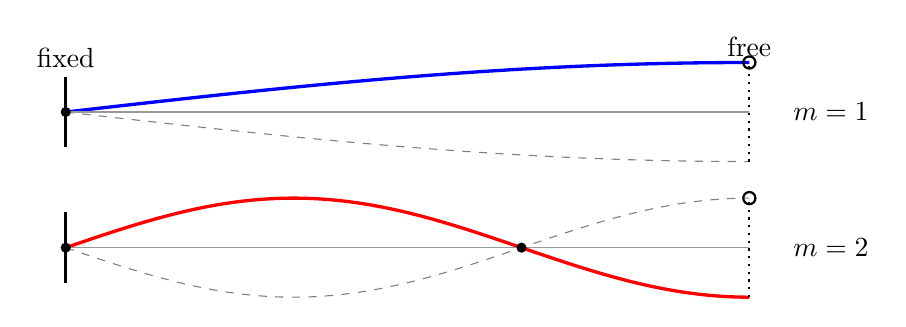
\begin{tikzpicture}
\begin{axis}[
    hide axis,
    width=12cm, height=6cm,
    xmin=-0.08, xmax=1.12, ymin=-2.20, ymax=0.75,
    samples=120, domain=0:1,
    clip=false,
]
    % m = 1 : quarter wave, node at 0, antinode at L
    \addplot[very thick, blue] {0.42*sin(deg(0.5*pi*x))};
    \addplot[gray, dashed] {-0.42*sin(deg(0.5*pi*x))};
    % m = 2 : (3/2) : node at 0, one interior node, antinode at L
    \addplot[very thick, red] {-1.15 + 0.42*sin(deg(1.5*pi*x))};
    \addplot[gray, dashed] {-1.15 - 0.42*sin(deg(1.5*pi*x))};
    % baselines, fixed wall at x=0, free rod at x=1
    \draw[thin, black!40] (axis cs:0,0) -- (axis cs:1,0);
    \draw[very thick] (axis cs:0,-0.30) -- (axis cs:0,0.30);
    \draw[thick, dotted] (axis cs:1,-0.42) -- (axis cs:1,0.42);
    \node[fill=black,circle,inner sep=1.3pt] at (axis cs:0,0) {};
    \draw[thin, black!40] (axis cs:0,-1.15) -- (axis cs:1,-1.15);
    \draw[very thick] (axis cs:0,-1.45) -- (axis cs:0,-0.85);
    \draw[thick, dotted] (axis cs:1,-1.57) -- (axis cs:1,-0.73);
    \node[fill=black,circle,inner sep=1.3pt] at (axis cs:0,-1.15) {};
    % free-end rings (antinodes)
    \draw[thick] (axis cs:1,0.42) circle[radius=2.2pt];
    \draw[thick] (axis cs:1,-1.15+0.42) circle[radius=2.2pt];
    % interior node of m=2 at x=2/3
    \node[fill=black,circle,inner sep=1.3pt] at (axis cs:0.6667,-1.15) {};
    % labels
    \node[anchor=west] at (axis cs:1.05,0) {$m=1$};
    \node[anchor=west] at (axis cs:1.05,-1.15) {$m=2$};
    \node[anchor=north] at (axis cs:0,0.62) {fixed};
    \node[anchor=north] at (axis cs:1,0.72) {free};
\end{axis}
\end{tikzpicture}
\caption{Standing waves on a string fixed at $x=0$ (node, filled dot) and free at $x=L$ (antinode, open ring sliding on the dotted rod). Only odd quarter-wavelengths fit: $\lambda_m = 4L/(2m-1)$.}
\label{fig:fixed-free}
\end{figure}

% ============================================================
\section{Initial Conditions and Fourier Series}
% ============================================================

The boundary conditions fix $k_m$ and $\alpha_m$; two further pieces of data --- the initial displacement $\psi(x,0)$ and the initial velocity $\dot\psi(x,0)$ --- are needed to pin down $A_m$ and $\beta_m$ for every mode. The remarkable fact, due to Fourier, is that \emph{any} reasonable initial shape can be written as a superposition of the normal modes, so this program always succeeds.

\subsection{Release from Rest}

Suppose the string is drawn into some shape and released from rest, so that $\dot\psi(x,0) = 0$ everywhere. Differentiating the modal expansion~\eqref{eq:normalmode} in $t$ and evaluating at $t=0$,
\begin{equation}
    \dot\psi_m(x,0) = A_m\,\omega_m\,\sin(k_m x + \alpha_m)\,\cos(\beta_m) = 0
    \quad\Longrightarrow\quad \cos\beta_m = 0.
\end{equation}
Choosing $\beta_m = -\pi/2$ turns $\sin(\omega_m t - \pi/2)$ into $-\cos(\omega_m t)$; absorbing the sign into $A_m$ leaves
\begin{equation}
    \psi_m(x,t) = A_m\,\sin(k_m x + \alpha_m)\,\cos(\omega_m t).
\end{equation}
The interpretation is clean: the amplitude $A_m$ encodes the shape at the moment of release, while the phase $\beta_m$ encodes the initial velocity distribution. Releasing from rest fixes every $\beta_m$ at once, leaving only the amplitudes to be determined.

\subsection{Orthogonality of Sinusoids}

The algebraic engine behind Fourier decomposition is the mutual \emph{orthogonality} of the mode shapes:
\begin{formula}
\begin{equation}
    \int_0^L \sin(k_m x)\,\sin(k_n x)\,\dd x = \begin{cases} L/2, & k_m = k_n, \\ 0, & k_m \neq k_n, \end{cases}
\end{equation}
\end{formula}
for the fixed-fixed wavenumbers $k_n = n\pi/L$. Two different modes are ``perpendicular'' in the sense of this inner product, so each acts as an independent axis in the space of shapes. Extracting the coefficient of one mode is then just a matter of projecting onto it.

\subsection{Extracting Fourier Coefficients}

Given an initial shape $f(x) = \psi(x,0)$ expanded over the modes,
\begin{equation}
    f(x) = \sum_{m=1}^{\infty} A_m \sin(k_m x),
\end{equation}
we project by multiplying both sides by $\sin(k_n x)$ and integrating over $[0,L]$. Orthogonality kills every term but one:
\begin{equation}
    \int_0^L \sin(k_n x)\,f(x)\,\dd x = \sum_{m=1}^\infty A_m \int_0^L \sin(k_n x)\sin(k_m x)\,\dd x = A_n\,\frac{L}{2}.
\end{equation}
Solving for the surviving coefficient,
\begin{formula}
\begin{equation}
    A_n = \frac{2}{L}\int_0^L \sin(k_n x)\,f(x)\,\dd x.
\end{equation}
\end{formula}
This is the Fourier sine series appropriate to a string with two fixed ends. For the mixed boundary condition (fixed at $x=0$, free at $x=L$) the identical projection argument, now with $k_n = (n-\tfrac{1}{2})\pi/L$, gives
\begin{equation}
    A_n = \frac{2}{L}\int_0^L \sin\!\left(\frac{(n-\tfrac{1}{2})\pi x}{L}\right)f(x)\,\dd x.
\end{equation}

\begin{example}[Rectangular initial displacement]
Take a piecewise-constant initial profile,
\begin{equation}
    f(x) = \begin{cases} 0, & x < aL, \\ h, & aL < x < bL, \\ 0, & x > bL, \end{cases}
\end{equation}
on a fixed-fixed string of length $L$, released from rest. With $k_n = n\pi/L$ the projection integral runs only over the raised interval,
\begin{equation}
    A_n = \frac{2}{L}\int_{aL}^{bL} h\,\sin(k_n x)\,\dd x = \frac{2h}{n\pi}\bigl(\cos(a n\pi) - \cos(b n\pi)\bigr).
\end{equation}
Assembling the modes with their time dependence gives the full solution,
\begin{equation}
    y(x,t) = \sum_{n=1}^\infty \frac{2h}{n\pi}\bigl(\cos(a n\pi) - \cos(b n\pi)\bigr)\sin\!\left(\frac{n\pi x}{L}\right)\cos\!\left(\frac{n\pi v_p t}{L}\right).
\end{equation}
As we will see from the traveling-wave viewpoint, this initial bump splits into equal left- and right-moving halves, each reflecting off the boundaries; because the medium is nondispersive ($\omega = v_p k$), the two halves reassemble perfectly at regular intervals and the motion repeats forever.
\end{example}

% ============================================================
\section{Fourier Series on $[-L, L]$}
% ============================================================

It is often more convenient to work on the symmetric interval $[-L, L]$, where the reflection symmetry $x \to -x$ organizes the modes by parity. The change of variables $x' = (x + L)/2$ maps the standard coordinate $x' \in [0, L]$ onto the symmetric one. For a fixed-fixed string released from rest, the modes in the $x'$ coordinate are $\sin(m\pi x'/L)$ with $k_m = m\pi/L$; substituting back,
\begin{equation}
    \psi(x, 0) = A_m\,\sin\!\left(\frac{m\pi(x+L)}{2L}\right) = A_m\,\sin\!\left(\frac{m\pi x}{2L} + \frac{m\pi}{2}\right).
\end{equation}
In the symmetric coordinate the wavenumber is $k_m = m\pi/(2L)$ and the phase is $\alpha_m = m\pi/2$.

\subsection{Odd and Even Modes}

Expanding the sine of a sum exposes the parity of each mode:
\begin{equation}
    \sin\!\left(\frac{m\pi x}{2L} + \frac{m\pi}{2}\right) = \sin\!\left(\frac{m\pi x}{2L}\right)\cos\!\left(\frac{m\pi}{2}\right) + \cos\!\left(\frac{m\pi x}{2L}\right)\sin\!\left(\frac{m\pi}{2}\right).
\end{equation}
For odd $m$ we have $\cos(m\pi/2) = 0$, so the mode is proportional to $\cos(m\pi x/2L)$, an \emph{even} function. For even $m$ we have $\sin(m\pi/2) = 0$, so the mode is proportional to $\sin(m\pi x/2L)$, an \emph{odd} function. The two parities never mix.

\begin{formula}
The general fixed-fixed solution on $[-L, L]$ splits cleanly by parity:
\begin{equation}
    \psi(x,t) = \sum_{m\,\text{even}} B_m\,\cos(\omega_m t)\,\sin\!\left(\frac{m\pi x}{2L}\right) + \sum_{m\,\text{odd}} C_m\,\cos(\omega_m t)\,\cos\!\left(\frac{m\pi x}{2L}\right).
\end{equation}
\end{formula}
The coefficients follow from the orthogonality of $\sin$ and $\cos$ over $[-L,L]$:
\begin{equation}
    B_m = \frac{1}{L}\int_{-L}^{L}\psi(x,0)\,\sin\!\left(\frac{m\pi x}{2L}\right)\dd x, \qquad
    C_m = \frac{1}{L}\int_{-L}^{L}\psi(x,0)\,\cos\!\left(\frac{m\pi x}{2L}\right)\dd x.
\end{equation}
The symmetry of the initial condition immediately tells us which family survives: an odd $\psi(x,0)$ excites only the $B_m$ (even $m$), while an even $\psi(x,0)$ excites only the $C_m$ (odd $m$). This parity bookkeeping is a valuable sanity check --- half the coefficients often vanish before any integral is done.

\subsection{A Useful Integration Trick}

Integrals of the form $\int x\,\cos(kx)\,\dd x$ crop up whenever the initial profile is piecewise linear, as for a plucked triangle wave. Rather than integrating by parts, it is quicker to differentiate a known integral under the parameter $k$:
\begin{equation}
    \int x\,\cos(kx)\,\dd x = \int \pdv{k}\,\sin(kx)\,\dd x = \pdv{k}\int\sin(kx)\,\dd x = \pdv{k}\!\left(-\frac{\cos(kx)}{k}\right) = \frac{x\sin(kx)}{k} + \frac{\cos(kx)}{k^2}.
\end{equation}
Applying the same move to $\sin(kx)$, or differentiating a second time in $k$, regenerates the whole standard table of Fourier-coefficient integrals with almost no bookkeeping.

\begin{example}[Two initial conditions]
Suppose (i) $\dot\psi(x,0) = 0$ (starting from rest) and (ii) $\psi(x,0)$ is a known shape. Condition (i) forces $\cos(\beta_m) = 0$, so $\beta_m = \pi/2$, and the displacement at $t=0$ is
\begin{equation}
    \psi(x, 0) = \sum_m A_m \sin(k_m x + \alpha_m).
\end{equation}
The projection formula then reads, for the two admissible phases,
\begin{align}
    \alpha_m = 0: &\qquad A_m = \frac{2}{L}\int \psi(x,0)\sin(k_m x)\,\dd x, \\
    \alpha_m = \tfrac{\pi}{2}: &\qquad A_m = \frac{2}{L}\int \psi(x,0)\cos(k_m x)\,\dd x.
\end{align}
The factor $2/L$ traces back to $\overline{\sin^2} = \overline{\cos^2} = 1/2$ averaged over any whole number of half-wavelengths, which makes the normalization integral equal to $L/2$.
\end{example}

% ============================================================
\section{Traveling Waves}
% ============================================================

Standing waves are one basis for solutions of the wave equation; \emph{traveling waves} are another. The two descriptions are related by trigonometric identities --- a standing wave is the sum of two oppositely moving traveling waves --- but they offer very different physical intuition. Where the standing-wave picture emphasizes the discrete spectrum of a bounded string, the traveling-wave picture makes the propagation of a localized pulse manifest.

\subsection{d'Alembert's Solution}

\begin{theorem}[d'Alembert]
Any twice-differentiable function of the single combination $x \pm v_p t$ solves the wave equation. Writing $\eta \defeq x - v_p t$, the chain rule gives
\begin{equation}
    \pdv{f}{x} = \pdv{f}{\eta}\,\pdv{\eta}{x} = \pdv{f}{\eta},\qquad
    \pdv{f}{t} = \pdv{f}{\eta}\,\pdv{\eta}{t} = -v_p\,\pdv{f}{\eta},
\end{equation}
so that
\begin{equation}
    \pdv[2]{f}{x} = \pdv[2]{f}{\eta}, \qquad \pdv[2]{f}{t} = v_p^{\,2}\,\pdv[2]{f}{\eta} \quad\Longrightarrow\quad \pdv[2]{f}{t} = v_p^{\,2}\,\pdv[2]{f}{x}. \checkmark
\end{equation}
The general solution of the 1D wave equation on the real line is therefore
\begin{equation}
    \psi(x,t) = f(x - v_p t) + g(x + v_p t),
\end{equation}
a right-moving pulse $f$ superposed on a left-moving pulse $g$, each rigidly preserving its shape.
\end{theorem}

For instance, a Gaussian $y = A\exp\bigl[-(x - v_p t)^2/(2\sigma^2)\bigr]$ is a rigid bump gliding to the right at speed $v_p$: replacing $t$ by $t + \Delta t$ simply shifts the whole profile a distance $v_p\,\Delta t$ downstream, without distortion.

\subsection{Matching Initial Conditions}

Given an initial displacement $y(x,0) = h(x)$ released from rest, $\dot y(x,0) = 0$, we determine the two d'Alembert pieces by evaluating $y = f(x - v_p t) + g(x + v_p t)$ and its time derivative at $t=0$:
\begin{align}
    y(x,0) &= f(x) + g(x) = h(x), \\
    \dot y(x,0) &= -v_p\,f'(x) + v_p\,g'(x) = 0 \;\Longrightarrow\; f'(x) = g'(x) \;\Longrightarrow\; f(x) = g(x).
\end{align}
Hence $f(x) = g(x) = h(x)/2$: an initial hump released from rest splits into two half-amplitude copies, one traveling in each direction (Figure~\ref{fig:dalembert}). This is exactly the microscopic mechanism behind the ``splitting and reassembling'' remark of the rectangular-pulse example above.

\begin{figure}[ht]
\centering
\begin{tikzpicture}[scale=1.0]
    % helper: a triangular pulse of half-width 0.5 and given height at (cx, base)
    % t = 0 : single full pulse
    \begin{scope}[yshift=4.2cm]
        \draw[thin, black!40] (0,0) -- (9,0);
        \draw[very thick, blue] (0,0) -- (4,0) -- (4.5,1) -- (5,0) -- (9,0);
        \node[anchor=east] at (-0.15,0.3) {$t=0$};
    \end{scope}
    % t = t1 : two half pulses just separated
    \begin{scope}[yshift=2.1cm]
        \draw[thin, black!40] (0,0) -- (9,0);
        \draw[very thick, red]  (0,0) -- (3,0) -- (3.5,0.5) -- (4,0) -- (5,0) -- (5.5,0.5) -- (6,0) -- (9,0);
        \draw[-{Latex}] (3.0,0.72) -- (2.3,0.72) node[anchor=east] {$g$};
        \draw[-{Latex}] (6.0,0.72) -- (6.7,0.72) node[anchor=west] {$f$};
        \node[anchor=east] at (-0.15,0.3) {$t=t_1$};
    \end{scope}
    % t = t2 : halves far apart
    \begin{scope}[yshift=0cm]
        \draw[thin, black!40] (0,0) -- (9,0);
        \draw[very thick, orange] (0,0) -- (1,0) -- (1.5,0.5) -- (2,0) -- (7,0) -- (7.5,0.5) -- (8,0) -- (9,0);
        \draw[-{Latex}] (1.0,0.72) -- (0.3,0.72);
        \draw[-{Latex}] (8.0,0.72) -- (8.7,0.72);
        \node[anchor=east] at (-0.15,0.3) {$t=t_2$};
    \end{scope}
\end{tikzpicture}
\caption{d'Alembert's construction. An initial pulse released from rest (top) splits into a left-moving half $g$ and a right-moving half $f$, each of half the original height. Successive snapshots ($t_1 < t_2$) show the two copies separating at speed $v_p$.}
\label{fig:dalembert}
\end{figure}

\subsection{Boundary Conditions on a Finite Interval}

On a finite string the traveling pulse eventually meets an end and reflects. The reflection rule follows from the same boundary conditions as before, now applied to the d'Alembert form.

\paragraph{Fixed end.} At $x=0$ write $y(x, t) = f(t - x/v_p) + f_R(t + x/v_p)$, an outgoing pulse plus its reflection. The clamp condition $y(0,t) = 0$ gives
\begin{equation}
    f(t) + f_R(t) = 0 \;\Longrightarrow\; f_R(t) = -f(t).
\end{equation}
A pulse striking a fixed end reflects \emph{inverted}.

\paragraph{Free end.} Now the condition $\pdv{y}{x}\big|_{x=0} = 0$ gives
\begin{equation}
    -\frac{1}{v_p}\,f'(t) + \frac{1}{v_p}\,f_R'(t) = 0 \;\Longrightarrow\; f'(t) = f_R'(t) \;\Longrightarrow\; f_R(t) = f(t).
\end{equation}
A pulse striking a free end reflects \emph{upright}.

These two rules suggest a tidy trick for the finite-interval initial-value problem: \emph{extend} the initial data outside $[0,L]$ so that the boundary conditions hold automatically --- an odd extension across each fixed end, an even extension across each free end --- and then let both copies propagate freely on the infinite line. The reflections take care of themselves, and restricting the resulting infinite-line solution back to $[0,L]$ recovers the answer.

% ============================================================
\section{Energy Transport in a Wave}
% ============================================================

A wave carries energy as well as displacement. To account for it, examine a small element of string and tally its kinetic and potential contributions. Consider a segment of length $\dd x$ and mass $\dd m = \rho_L\,\dd x$ moving with transverse velocity $\pdv{y}{t}$; its kinetic energy is
\begin{equation}
    \dd(KE) = \tfrac{1}{2}\,\dd m\,\!\left(\pdv{y}{t}\right)^2 = \tfrac{1}{2}\,\rho_L\!\left(\pdv{y}{t}\right)^2 \dd x,
\end{equation}
so the total kinetic energy on a string of length $L$ is
\begin{formula}
\begin{equation}
    KE = \int_0^L \tfrac{1}{2}\,\rho_L\!\left(\pdv{y}{t}\right)^2 \dd x.
\end{equation}
\end{formula}

\subsection{Potential Energy of a Stretched String}

The potential energy is the work stored in stretching the string against its tension. A displaced element occupies more arclength than its horizontal footprint $\dd x$, and it is that extra length, pulled taut against $T$, which holds the energy. Referring to the element of Figure~\ref{fig:element}, an element of horizontal extent $\dd x$ with vertical rise $\dd y$ has arclength $\sqrt{\dd x^2 + \dd y^2}$, so the stretch is
\begin{equation}
    \dd s = \sqrt{\dd x^2 + \dd y^2} - \dd x = \dd x\!\left(\sqrt{1 + \left(\pdv{y}{x}\right)^2} - 1\right) \approx \tfrac{1}{2}\!\left(\pdv{y}{x}\right)^2 \dd x,
\end{equation}
using $(1+u)^{1/2} \approx 1 + u/2$ for small slope. The work done against tension is $\dd W = T\,\dd s$, and integrating,
\begin{formula}
\begin{equation}
    PE = \int_0^L \tfrac{1}{2}\,T\!\left(\pdv{y}{x}\right)^2 \dd x.
\end{equation}
\end{formula}
Notice that the potential energy density is controlled by the \emph{slope} of the string. A sharp corner, with its large local slope, stores more energy than a gently bulged profile of the same displacement --- the microscopic reason that string vibrations tend to smooth themselves out, and that a high harmonic carries more energy than the fundamental at equal amplitude.

\begin{figure}[ht]
\centering
\begin{tikzpicture}[scale=1.5]
    % curved string element
    \draw[thick, black!30] (-1.1,-0.30) .. controls (-0.4,0.05) and (0.2,0.55) .. (1.6,1.15);
    \draw[very thick, blue] (0,0.18) .. controls (0.35,0.36) and (0.65,0.58) .. (1.0,0.86);
    % tangent tension vectors
    \draw[-{Latex}, thick] (0,0.18) -- ++(-0.62,-0.31) node[anchor=north east] {$T$};
    \draw[-{Latex}, thick] (1.0,0.86) -- ++(0.66,0.55) node[anchor=south west] {$T$};
    % horizontal dashed references at the two ends
    \draw[dashed, black!55] (0,0.18) -- ++(0.5,0);
    \draw[dashed, black!55] (1.0,0.86) -- ++(0.5,0);
    % angles
    \draw (0.30,0.18) arc[start angle=0, end angle=27, radius=0.30] ;
    \node at (0.44,0.30) {$\theta_1$};
    \draw (1.30,0.86) arc[start angle=0, end angle=40, radius=0.30];
    \node at (1.46,1.02) {$\theta_2$};
    % dx and dy braces
    \draw[dotted] (0,0.18) -- (1.0,0.18);
    \draw[dotted] (1.0,0.18) -- (1.0,0.86);
    \draw[|<->|] (0,-0.10) -- (1.0,-0.10) node[midway,below] {$\dd x$};
    \draw[|<->|] (1.28,0.18) -- (1.28,0.86) node[midway,right] {$\dd y$};
\end{tikzpicture}
\caption{A displaced element of string (blue) of horizontal extent $\dd x$ and rise $\dd y$. The tension $T$ pulls tangentially at each end, making angles $\theta_1$ and $\theta_2$ with the horizontal; the small difference $\theta_2 - \theta_1$ supplies the transverse restoring force, and the extra arclength stores the potential energy.}
\label{fig:element}
\end{figure}

\begin{example}[Total energy of a Gaussian pulse]
For the traveling Gaussian $y(x,t) = y_0\,\exp\!\bigl[-(x-v_p t)^2/(2\sigma^2)\bigr]$, differentiation gives
\begin{equation}
    \pdv{y}{t} = \frac{y_0 v_p (x - v_p t)}{\sigma^2}\exp\!\left[-\frac{(x-v_pt)^2}{2\sigma^2}\right], \qquad \pdv{y}{x} = -\frac{1}{v_p}\pdv{y}{t}.
\end{equation}
The kinetic-energy density is $\varepsilon_K = \tfrac{1}{2}\rho_L(\partial_t y)^2$, and using $v_p^2 = T/\rho_L$ the potential-energy density is $\varepsilon_P = \tfrac{1}{2}T(\partial_x y)^2 = \tfrac{1}{2}\rho_L(\partial_t y)^2 = \varepsilon_K$. Energy is thus equipartitioned between kinetic and potential form at \emph{every} point of a traveling wave --- a hallmark of nondispersive propagation. Substituting $u = (x-v_pt)/\sigma$,
\begin{equation}
    KE = \frac{\rho_L y_0^2 v_p^2}{2\sigma}\int_{-\infty}^{\infty} u^2 e^{-u^2}\,\dd u = \frac{\rho_L y_0^2 v_p^2 \sqrt{\pi}}{4\sigma},
\end{equation}
and by equipartition $E = KE + PE = 2\,KE = T y_0^2\sqrt{\pi}/(2\sigma)$. A narrower pulse (smaller $\sigma$) carries \emph{more} energy at fixed height, because its slopes are steeper.
\end{example}

\begin{example}[Power carried by a traveling wave]
The power crossing a fixed station $x_0$ equals the transverse force the string exerts on its right neighbour times that neighbour's transverse velocity: $P(x_0,t) = -T\sin\theta\,\partial_t y \approx -T\,\partial_x y\,\partial_t y$ for small slopes. For the Gaussian above, using $\partial_x y = -\partial_t y/v_p$,
\begin{equation}
    P(x_0,t) = \frac{T}{v_p}\,(\partial_t y)^2 = \frac{v_p T\,y_0^2 (x_0 - v_pt)^2}{\sigma^4}\exp\!\left[-\frac{(x_0-v_pt)^2}{\sigma^2}\right].
\end{equation}
The power is manifestly non-negative --- energy always flows in the direction of propagation --- and its time integral $\int_{-\infty}^{\infty} P\,\dd t$ equals the total pulse energy found above, confirming that nothing is lost in transit.
\end{example}

% ============================================================
\section{Reflection and Transmission at a Density Boundary}
% ============================================================

What happens when a wave meets an abrupt change in the medium? Join two semi-infinite strings at $x=0$ with a massless bead of glue. The left string has density $\rho_{L,L}$ and the right has $\rho_{L,R}$; both carry the same tension $T$, so their wave speeds differ,
\begin{equation}
    v_L = \sqrt{T/\rho_{L,L}}, \qquad v_R = \sqrt{T/\rho_{L,R}}.
\end{equation}
An incoming pulse $f_i(x - v_L t)$ arriving from the left will in general partially \emph{reflect}, as a left-mover $f_R(x + v_L t)$, and partially \emph{transmit}, as a right-mover $f_T(x - v_R t)$ in the new medium (Figure~\ref{fig:reftrans}).

\begin{figure}[ht]
\centering
\begin{tikzpicture}[scale=1.0]
    % junction
    \draw[dashed, black!50] (0,-1.0) -- (0,1.0);
    \node[anchor=south] at (0,1.0) {$x=0$};
    % left (light) string
    \draw[thick] (-5,0) -- (0,0);
    \node[anchor=north] at (-3.4,-0.18) {light: $\rho_{L,L}$, $v_L$};
    % right (heavy) string
    \draw[line width=2.2pt] (0,0) -- (5,0);
    \node[anchor=north] at (2.6,-0.15) {heavy: $\rho_{L,R}$, $v_R$};
    % incident bump (up), moving right
    \draw[very thick, blue] (-4.5,0) -- (-3.7,0) -- (-3.3,0.7) -- (-2.9,0) -- (-1.5,0);
    \draw[-{Latex}, blue] (-3.9,0.9) -- (-3.0,0.9) node[anchor=west] {incident};
    % reflected bump (inverted, moving left)
    \draw[very thick, red] (-1.5,0) -- (-1.1,0) -- (-0.7,-0.4) -- (-0.3,0) -- (0,0);
    \draw[-{Latex}, red] (-0.5,-0.60) -- (-1.15,-0.60);
    \node[red, anchor=north] at (-0.85,-0.92) {reflected};
    % transmitted bump (up, moving right, stretched a bit lower)
    \draw[very thick, orange] (0,0) -- (1.6,0) -- (2.4,0.5) -- (3.2,0) -- (4.5,0);
    \draw[-{Latex}, orange] (2.0,0.7) -- (2.9,0.7) node[anchor=west] {transmitted};
\end{tikzpicture}
\caption{A pulse incident from a light string (thin) onto a heavier string (thick), joined at $x=0$. Part reflects --- inverted here because $v_R < v_L$ --- and part transmits into the slower medium, where it is broader and shorter.}
\label{fig:reftrans}
\end{figure}

\subsection{Boundary Conditions at the Junction}

\begin{fact}
Two conditions hold at the junction $x=0$:
\begin{enumerate}
    \item \emph{Continuity of displacement} --- the string does not break:
    \begin{equation}
        y_L(0,t) = y_R(0,t).
    \end{equation}
    \item \emph{Force balance on the massless bead} --- with $m_{\text{glue}}=0$ the net transverse force must vanish. For small angles $\sin\theta \approx \pdv{y}{x}$, so the slopes match:
    \begin{equation}
        \left.\pdv{y_L}{x}\right|_{x=0} = \left.\pdv{y_R}{x}\right|_{x=0}.
    \end{equation}
\end{enumerate}
\end{fact}

A third observation ties the two sides together: because the bead is a single point shared by both strings, its two faces must oscillate at a \emph{common} frequency $\omega$. Since $\omega = v k$ is preserved across the junction while $v$ jumps, the wavenumber must jump too: $v_L k_L = v_R k_R = \omega$.

\subsection{Reflection and Transmission Coefficients}

Write the reflected and transmitted amplitudes as constant multiples of the incident one,
\begin{equation}
    f_R(u) = R\,f_i(u), \qquad f_T(u) = T\,f_i(u),
\end{equation}
so that $R$ and $T$ are two unknowns to be fixed by the two boundary conditions. Continuity of displacement at $x=0$ gives
\begin{equation}
    f_i(\omega t) + R\,f_i(\omega t) = T\,f_i(\omega t) \;\Longrightarrow\; 1 + R = T.
\end{equation}
Continuity of slope, using $\pdv{f}{x} = -\tfrac{1}{v}\,\pdv{f}{t}$ for a right-mover and $\pdv{f}{x} = +\tfrac{1}{v}\,\pdv{f}{t}$ for a left-mover, gives after simplification
\begin{equation}
    \frac{1}{v_L}(R - 1) = -\frac{1}{v_R}\,T.
\end{equation}
Solving the pair simultaneously,
\begin{formula}
\begin{equation}
    R = \frac{v_R - v_L}{v_R + v_L}, \qquad T = \frac{2 v_R}{v_R + v_L}.
\end{equation}
\end{formula}
It is cleaner still to phrase the result in terms of the \emph{mechanical impedance} $Z \defeq \sqrt{T\rho_L} = T/v$, which is the property the boundary really cares about:
\begin{equation}
    R = \frac{Z_L - Z_R}{Z_L + Z_R}, \qquad T = \frac{2 Z_L}{Z_L + Z_R}.
\end{equation}

\subsection{Limits and Observations}

A few limits bring these formulae to life. When $v_R = v_L$ (equivalently $Z_L = Z_R$) the reflection coefficient vanishes: an impedance-matched junction transmits everything and reflects nothing, the principle behind anti-reflection coatings and impedance-matching transformers. Driving the right medium to infinite density, $\rho_{L,R}\to\infty$, sends $v_R \to 0$, so $T \to 0$ and $R \to -1$; the transmitted wave dies while the reflected wave returns fully inverted, exactly reproducing the fixed-end limit. Finally, since $\omega$ is preserved but $v$ is not, the wavelength $2\pi/k = 2\pi v/\omega$ stretches on entering a faster medium and compresses on entering a slower one --- the pulse is geometrically rescaled as it crosses.

\begin{example}[Reflection and transmission at a tension boundary]
Consider instead two semi-infinite strings of common density $\rho$ but different tensions $T_1$ (left) and $T_2$ (right), joined at $x=0$. An incident wave $\psi_i = \alpha\cos(kx - \omega t)$ arrives from the left. Because $\omega$ is common while $v_i = \sqrt{T_i/\rho}$ differs, the transmitted wavenumber is $k_2 = \sqrt{T_1/T_2}\,k$.

Take the ansatz $\psi_r = R\alpha\cos(-kx - \omega t)$ for the reflected wave and $\psi_t = T\alpha\cos(\sqrt{T_1/T_2}\,kx - \omega t)$ for the transmitted wave. Continuity of displacement at $x=0$ yields $1 + R = T$. Force balance on the massless junction, $T_2\,\partial_x\psi_t = T_1\,\partial_x(\psi_i+\psi_r)$ at $x=0$, gives after simplification $T = \sqrt{T_1/T_2}\,(1-R)$. Solving the pair,
\begin{equation}
    R = \frac{\sqrt{T_1/T_2} - 1}{\sqrt{T_1/T_2} + 1}, \qquad T = \frac{2\sqrt{T_1/T_2}}{\sqrt{T_1/T_2}+1}.
\end{equation}
These mirror the density-boundary formulae exactly, as they must: the mechanical impedance $Z = \sqrt{T\rho}$ is the sole arbiter, so raising $T$ at fixed $\rho$ plays the same role as lowering $\rho$ at fixed $T$. The instantaneous power delivered across $x=0$, $P = -T_1\,\partial_x\psi_1\,\partial_t\psi_1$, is continuous across the junction --- as it must be, since the massless bead stores no energy.
\end{example}

% ============================================================
\section{Summary}
% ============================================================

\begin{fact}[Wave equation cheat sheet]\hfill

\textbf{Wave equation:} $\pdv[2]{\psi}{t} = v_p^{\,2}\,\pdv[2]{\psi}{x}$ with dispersion $\omega = v_p |k|$.

\textbf{Wave speeds:} string, $v_p = \sqrt{T/\rho_L}$; sound, $v_p = \sqrt{\gamma p_0/\rho}$; EM, $v_p = c = 1/\sqrt{\mu_0\varepsilon_0}$.

\textbf{Normal-mode solution:} $\psi(x,t) = \sum_m A_m \sin(k_m x + \alpha_m)\sin(\omega_m t + \beta_m)$.

\textbf{Boundary conditions:}
\begin{itemize}
    \item Closed (fixed): $y(x_b, t) = 0$.
    \item Open (free): $\left.\pdv{y}{x}\right|_{x_b} = 0$.
\end{itemize}

\textbf{Traveling-wave solution:} $\psi(x, t) = f(x - v_p t) + g(x + v_p t)$, with reflection rules
\begin{itemize}
    \item Closed: inverted reflection, $f_R = -f$.
    \item Open: upright reflection, $f_R = +f$.
\end{itemize}

\textbf{Density boundary:} $1 + R = T$; $\;R = (v_R - v_L)/(v_R + v_L)$; $\;T = 2 v_R/(v_R + v_L)$.

\textbf{Energies:}
\begin{equation*}
    KE = \tfrac{1}{2}\rho_L \int_0^L \!\left(\pdv{\psi}{t}\right)^2 \dd x, \qquad PE = \tfrac{1}{2}T\int_0^L \!\left(\pdv{\psi}{x}\right)^2 \dd x.
\end{equation*}

\textbf{Handy integrals:} $\int_0^\ell \sin^2(\tfrac{\pi}{c}x)\,\dd x = \int_0^\ell \cos^2(\tfrac{\pi}{c}x)\,\dd x = \ell/2$ over any whole number of half-periods.
\end{fact}

% ============================================================
\section{Sound Waves}
% ============================================================

Longitudinal pressure waves obey the same wave equation, now with $\psi(x,t)$ the local particle displacement and the pressure fluctuation given by
\begin{equation}
    P(x,t) = P_0 + \Delta P(x,t), \qquad \Delta P(x,t) = -\gamma P_0\,\pdv{\psi}{x}.
\end{equation}
The boundary conditions for a pipe distinguish a mechanically clamped end from an end open to the atmosphere, and the two cases exchange the roles of displacement and pressure. At a closed end (a rigid wall) the gas cannot move, so $\psi(x_0,t) = 0$ --- a displacement node. Since $\Delta P \propto -\partial_x\psi$, the displacement gradient need not vanish there; in fact it is maximal, so the pressure fluctuation sits at an antinode. At an open end the gas is free to slosh in and out, but the pressure must match the atmosphere, so $\Delta P(x_0,t) = 0$ and hence $\partial_x\psi|_{x_0} = 0$ --- a pressure node and a displacement antinode. This systematic swap between displacement- and pressure-behaviour at the two boundary types is precisely why open and closed pipes of the same length sound different fundamental pitches.

% ============================================================
\section{Electromagnetic Waves}
% ============================================================

In vacuum, Maxwell's equations decouple into wave equations for $\vect{E}$ and $\vect{B}$ separately:
\begin{equation}
    \pdv[2]{\vect{E}}{t} = \frac{1}{\mu_0\varepsilon_0}\,\laplacian\vect{E}, \qquad
    \pdv[2]{\vect{B}}{t} = \frac{1}{\mu_0\varepsilon_0}\,\laplacian\vect{B},
\end{equation}
both propagating at the speed of light $c = 1/\sqrt{\mu_0\varepsilon_0}$. A plane wave is specified by a wave vector $\vect{k} = (k_x, k_y, k_z)$, so that $\vect{r}\cdot\vect{k} = k_x x + k_y y + k_z z$, together with a polarization direction for $\vect{E}$.

\begin{formula}[Traveling EM plane wave]
For $\vect{E}(\vect{r}, t) = E_0\,\uvect{x}\cos(kz - \omega t)$, Faraday's law $\curl\vect{E} = -\pdv{\vect{B}}{t}$ gives
\begin{equation}
    \vect{B}(\vect{r}, t) = \frac{1}{c}\,\uvect{k}\times\vect{E}(\vect{r}, t).
\end{equation}
The three vectors form a right-handed triad with propagation direction $\uvect{k} = \uvect{E}\times\uvect{B} = \frac{1}{\|\vect{k}\|}\bigl(\vect{E}\times\vect{B}\bigr)$.
\end{formula}

\subsection{Boundary Conditions and Energy}

At a perfect conductor the tangential electric field must vanish, $\vect{E}(\vect{r}_b, t) = 0$ on the boundary --- the electromagnetic analog of a clamped string end. For a standing EM wave, $\vect{E}$ and $\vect{B}$ are then $90^\circ$ out of phase in both space and time: the magnetic field is largest where the electric field vanishes, and vice versa.

The energy densities are
\begin{equation}
    u_E = \tfrac{1}{2}\varepsilon_0 E^2, \qquad u_B = \frac{1}{2\mu_0}B^2,
\end{equation}
and the energy current --- power per unit area --- is the \emph{Poynting vector}:
\begin{formula}
\begin{equation}
    \vect{S} = \frac{\vect{E}\times\vect{B}}{\mu_0}.
\end{equation}
\end{formula}
For a plane wave $\vect{S}$ points along $\uvect{k}$, with magnitude equal to the total (electric plus magnetic) energy density times $c$: the energy streams along at the wave speed, exactly as the traveling-wave picture would lead us to expect.
